\documentclass{aa}
\usepackage[varg]{txfonts}
%\usepackage[nottoc]{tocbibind}
%\usepackage[english]{babel}
%\usepackage[utf8]{inputenc}
%\usepackage{graphicx}
%\usepackage{amsmath,amssymb,amsfonts}
%\usepackage{geometry}
%\usepackage{paralist}
%\usepackage{color}
%\usepackage{fancyhdr}
%\usepackage{tikz}
%\usepackage{tikz-cd}
\usepackage{subfig}
%\usepackage[section]{placeins}
\usepackage{float}
\usepackage{booktabs}
\usepackage{bm}
\usepackage{siunitx}
%\usepackage{listings}
%\usepackage{natbib}
\bibpunct{(}{)}{;}{a}{}{,} % to follow the A&A style
%\citestyle{aa}
%\usepackage{biblatex}
%\usepackage{subfig}
%\usepackage{hyperref}
%\usepackage{gensymb}
%\usepackage{comment}
%\usepackage{longtable}
%\pagestyle{fancy}
%\fancyhead[L]{Optical Astronomy\\
%University of Bonn -- Winter Term 2016/17}
%\fancyhead[R]{Sven Heydenreich\\Antonio P\'erez Ib\'a\~nez}
%\cfoot{Page \thepage\ of \pageref{lastpage}}
\def\Msun{\ensuremath{\rm M_\odot}}
\def\Lsun{\ensuremath{L_\odot}}
\def\Rsun{\ensuremath{R_\odot}}
\def\inv{^{-1}}
\def\({\left(}
\def\r){\right)}
\def\b#1{\bm{#1}}
\def\Dd{D_{\text{d}}}
\def\Dds{D_{\text{ds}}}
\def\Ds{D_{\text{s}}}

%%% Notes
\usepackage{todonotes}
\newcommand{\antonio}[1]{\todo[color=green]{#1}}
\newcommand{\sven}[1]{\todo[color=orange]{#1}}
%\usepackage{hyperref}
\begin{document}
\title{The Abundance of primordial Black Holes from Quasar Microlensing}
\author{Evencio ~Mediavilla\inst{3,4}
\and Sven ~Heydenreich\inst{5}
\and Jorge ~Jim\' enez-Vincente\inst{1,2}}
\institute{Departamento de F\' isica Te\' orica y del Cosmos, Universidad de Granada, Campus de
Fuentenueva, E-18071 Granada, Spain
\and Instituto Carlos I de F\' isica Te\' orica y Computacional, Universidad de Granada, E-18071 Granada, Spain
\and Instituto de Astrof\' isica de Canarias, E-38200 La Laguna, Santa Cruz de Tenerife, Spain
\and Departamento de Astrof\' isica, Universidad de La Laguna, E-38200 La Laguna, Santa Cruz
de Tenerife, Spain
\and Argelander Institute for Astronomy, University of Bonn, Auf dem H\" ugel 71, 53121 Bonn, Germany
}
\abstract {The nature of Dark Matter is still an open debate. While a new elementary particle is the favoured hypothesis, MACHOs are still not ruled out as a candidate.}{We want to check whether clustered primordial black holes with masses of about $30\Msun$ are a reasonable candidate for Dark Matter.} {We will use single-time observations of 20 multiply-imaged quasars and compare those to simulations.}{We find that previous microlensing experiments do not rule out the existence of clustered primordial black holes: While the magnification probability of the continuum source is relatively insensitive to clustering of the lenses, the magnification behaviour of the broad line emission region, commonly used as a baseline, is strongly affected by the clusters. Also, our experiment shows that ...(tba)} {}
\maketitle
\section{Introduction}
Fueled by the lack of detection for elementary particles as suitable candidates for dark matter and by the recent detections of the LIGO-Observatory \citep{2017PhRvL.118v1101A,2016PhRvL.116x1103A,2017PhRvL.119n1101A,2016PhRvL.116f1102A,2017ApJ...851L..35A}, the hypothesis that Dark Matter consists of MAssive Compact Halo Objects (MACHOs) has received new popularity. Especially primordial black holes in the intermediate mass range (\SIrange{1}{1000}{\Msun}) are a favoured candidate, as their abundance is not constrained by the baryon fraction determined in the CMB analysis by the PLANCK-collaboration \citep{PhysRevD.94.083504,2016A&A...594A..13P}. \citet{2009ApJ...706.1451M} found that quasar microlensing provides an excellent method to analyze the fraction of compact objects in lens galaxies and used this method to check whether the existence of primordial black holes in said mass range is plausible \citep{2017ApJ...836L..18M}. However, instead of a uniform lens distribution, which is commonly assumed in microlensing experiments \citep{1999AAS...195.4802B,2015ApJ...806..251J}, we will adapt the physically motivated assumption that primordial black holes are clustered, where each cluster contains \numrange{100}{1000} black holes and has collapsed to sub-parsec scales \citep{2017arXiv171004694G}.
\section{Observations}
We used an inverse polygon mapping algorithm \citep{2011ApJ...741...42M,2006ApJ...653..942M} to construct magnification maps for each of the respective quasar images. We have no prior knowledge on the radial profile of clustered black holes, but a comparison of different profiles showed that the microlensing statistics are insensitive to the radial profile, so for simplicity we adapted a gaussian profile with variance $\sigma$ (\SIlist{0.1;0.2;0.4}{pc}). We also parametrized the number of black holes per cluster $N_{\rm BH}$ (\numlist{100;300;1000}) and the fraction of mass in microlenses (\numlist{0.0625;0.125;0.25;0.5;0.75;1.0}). We chose the masses of the black holes to be \SI{30}{\Msun}, which is in rough agreement both with the LIGO-observations and with \citet{2017arXiv171004694G}. In reality the mass profile would be more complex (\citet{2017arXiv171004694G} suggested a lognormal profile), but microlensing is only weakly sensitive to the slope of the mass spectrum; the only important quantity is the average mass \citep{2007MNRAS.376..263C}. For the continuum emission region we adapted a gaussian luminosity profile with a half-light radius of $\sigma = 2.5\, \text{lightdays}$ \citep{2016ApJ...821...56F,2009ApJ...706.1451M}. Again, the important quantity is only the half-light radius and not the luminosity profile itself \citep{2005ApJ...628..594M}. For each point in our parameter space we extracted a magnification histogram for the continuum region by convolving the magnification map with the source luminosity function and extracting the resulting histogram.

To compare the simulations with the observations we need to separate the magnification by microlensing from the magnification by the macro lens. This is done by establishing a \emph{baseline} of magnification (usually, the broad-line emission region is used for that \citep{2009ApJ...706.1451M}). Then we divide the flux of the continuum region by the baseline and compute the difference (in magnitudes) between the brightness of two separate images. In our simulations, this corresponds to a cross-correlation of the magnification histograms of the two images. In the end we can extract a likelihood function for the chosen parameters by applying Bayes' Theorem.
\section{Results}
We found that the magnification histograms, both the single and the cross-correlated ones, do not significantly differ from the unclustered case. Furthermore, the histograms are insensitive to both parameters $N_{\rm BH}$ and $\sigma$. However, we found that the magnification maps of clustered lenses are dominated by huge caustics caused by the clusters of black holes: To a light-ray passing outside of a cluster the whole cluster acts as a single lens with the mass of all the black holes combined. As the fraction of area taken by the clusters is relatively small, the features caused by the clusters dominate over the ones caused by single black holes. This strongly aggravates the determination of a baseline: Normally the broad line emission region is large enough that any microlensing effect is `washed out', i.e. the BLR is insensitive to microlensing. However, we are dealing with black holes whose masses are about \num{100} times larger than the ones of average stars. A cluster of \num{1000} of those black holes now induces features that are about \num{300} times larger and affect the BLR almost as much as thez affect the continuum source. A graphic representation of this can be found in Figure \ref{fig:relmag}.
\begin{figure*}
	\centering
	\subfloat[Uniform Distribution of Black Holes]{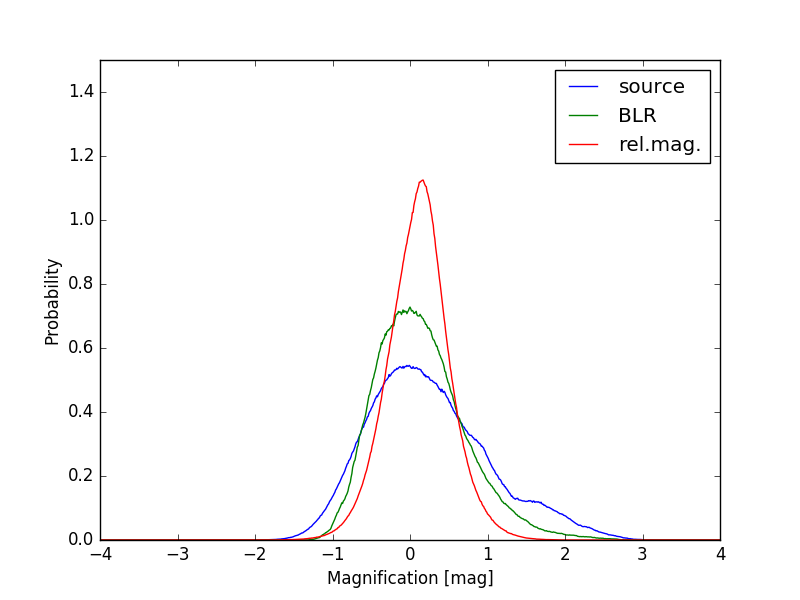
\includegraphics[width=0.5\textwidth]{imgs/unimagcomparison.png}}
	\subfloat[Clustered Distribution of Black Holes]{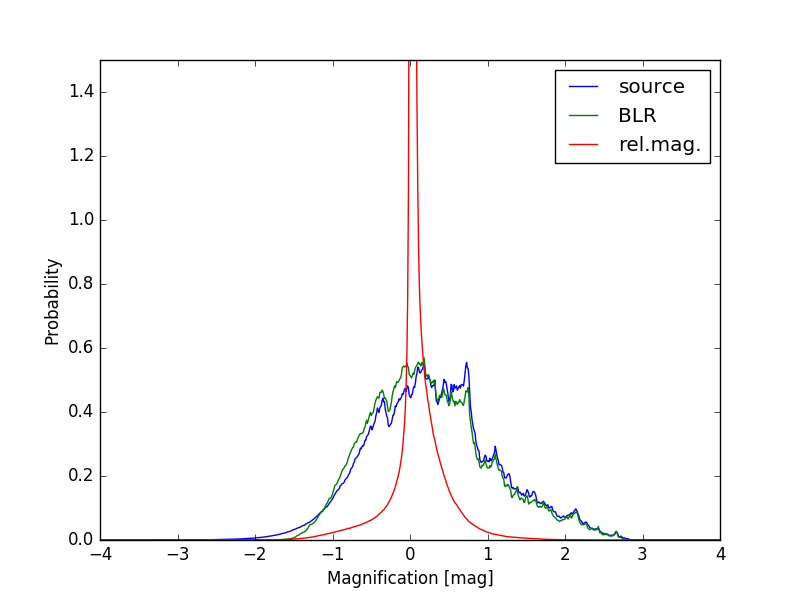
\includegraphics[width=0.5\textwidth]{imgs/clmagcomparison.png}}
	\caption{Magnification Histograms of the continuum emission region (blue line, corresponding to \SI{5}{lightdays}), the broad line emission region (green line, corresponding to \SI{30}{lightdays}) and the magnification of the continuum region divided by the broad line region (red line) in the uniform and the clustered case.}
	\label{fig:relmag}
\end{figure*}
Considering this, we can already formulate our first result: Microlensing experiments that compute the baseline using the broad-line emission region do not detect any effects of clustered primordial black holes, as the baseline is magnified almost as much as the continuum region. Results that exclude the existence of primordial black holes due to lack of observed microlensing (like \citet{2017ApJ...836L..18M}) do not apply to the case of clustered primordial black holes: A new study using a different method of baseline determination is necessary to exclude these.
\section{Discussion}

\section{Conclusion}
\bibliographystyle{aa}
\bibliography{cite}
\end{document}